\section{Piston}\label{piston}

\begin{figure}
\centering
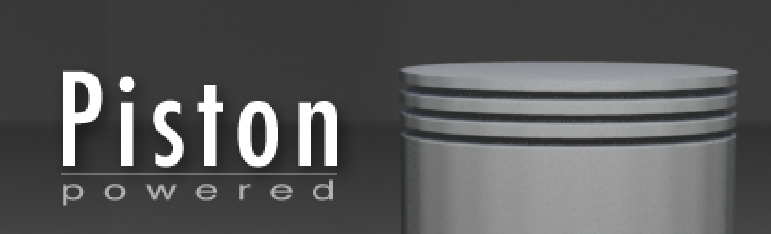
\includegraphics{images/piston}
\caption{Logo Pistonu \autocite{pistonpic}\label{pic:piston}}
\end{figure}

Piston je, respektive spíše byl, mini-framework pro Django určený pro vytváření RESTful API \autocite{piston}.

Piston je interně svázán s~Djangem a podle své dokumentace nabízí následující funkce \autocite{piston}:

\begin{itemize}
\tightlist
\item
  podporuje OAuth bez nutnosti použití další knihovny,
\item
  nevyžaduje vazbu na modely, umožňuje vytvářet nezávislé zdroje,
\item
  komunikuje pomocí JSONu, YAMLu, Python picklu a XML (a také pomocí HATEOAS),
\item
  jde o~Python knihovnu, kterou lze snadno použít,
\item
  respektuje a nabádá ke správnému využití HTTP protokolu (návratové kódy apod.),
\item
  má zabudovanou (volitelnou) validaci vstupů (pomocí Djanga), omezování počtu požadavků v~čase apod.,
\item
  podporuje streamování s~malým využitím paměti,
\item
  „neplete se do cesty“.
\end{itemize}

Projekt vnikl již v~roce 2008, tedy tři roky po zveřejnění Djanga samotného, pod záštitou Bitbucketu. V~roce 2010 jej však původní autor, Jesper Nøhr, přestal vyvíjet. Vývoje se následující rok ujal Joshua Ginsberg, který ale vydal jen dvě nové verze a vývoj na začátku roku 2012 taktéž opustil. Poslední vydaná verze 0.2.3 přidává podporu pro Django 1.4, nejvyšší podporovaná verze je tedy snad 1.5\footnote{Django vždy nejprve označí funkcionalitu k~odebrání, v~následující verzi ji označí jako zastaralou (\emph{deprecated}) a v~další verzi ji odstraní \autocite{djangorelease}. Současné podporované verze jsou 1.8 a 1.9.}. S~Djangem 1.6 nebo vyšším Piston nefunguje \autocite{piston16}. Kód rovněž obsahuje syntaxi nekompatibilní s~Pythonem 3. Piston je tedy jednoznačně mrtvý projekt.

Piston byl distribuován pod BSD licencí (není však jasné, jestli jde o~třípoložkovou \autocite{BSD3} nebo dvoupoložkovou \autocite{BSD2} variantu, projekt neuvádí celý text licence). Závisí pouze na Djangu a společně s~Djangem 1.5 má 75~311 řádků kódu.

Příklad použití z~dokumentace můžete vidět \protect\hyperlink{code:piston1}{v~ukázkách} \protect\hyperlink{code:piston2}{a}.

\begin{listing}[htbp]
\caption{{\label{code:piston1}Příklad použití z~dokumentace Pistonu (urls.py) \autocite{piston}}}
\begin{minted}[bgcolor=codebg]{python}
from django.conf.urls.defaults import *
from piston.resource import Resource
from piston.authentication import HttpBasicAuthentication

from myapp.handlers import BlogPostHandler, ArbitraryDataHandler

auth = HttpBasicAuthentication(realm="My Realm")
ad = { 'authentication': auth }

blogpost_resource = Resource(handler=BlogPostHandler, **ad)
arbitrary_resource = Resource(handler=ArbitraryDataHandler, **ad)

urlpatterns += patterns('',
    url(r'^posts/(?P<post_slug>[^/]+)/$', blogpost_resource), 
    url(r'^other/(?P<username>[^/]+)/(?P<data>.+)/$',
        arbitrary_resource), 
)
\end{minted}
\end{listing}

\begin{listing}[htbp]
\caption{{\label{code:piston2}Příklad použití z~dokumentace Pistonu (handlers.py) \autocite{piston}}}
\begin{minted}[bgcolor=codebg]{python}
import re

from piston.handler import BaseHandler
from piston.utils import rc, throttle

from myapp.models import Blogpost

class BlogPostHandler(BaseHandler):
    allowed_methods = ('GET', 'PUT', 'DELETE')
    fields = ('title', 'content',
              ('author', ('username', 'first_name')), 'content_size')
    exclude = ('id', re.compile(r'^private_'))
    model = Blogpost

    @classmethod
    def content_size(self, blogpost):
        return len(blogpost.content)

    def read(self, request, post_slug):
        post = Blogpost.objects.get(slug=post_slug)
        return post

    @throttle(5, 10*60) # allow 5 times in 10 minutes
    def update(self, request, post_slug):
        post = Blogpost.objects.get(slug=post_slug)

        post.title = request.PUT.get('title')
        post.save()

        return post

    def delete(self, request, post_slug):
        post = Blogpost.objects.get(slug=post_slug)

        if not request.user == post.author:
            return rc.FORBIDDEN # returns HTTP 401

        post.delete()

        return rc.DELETED # returns HTTP 204

class ArbitraryDataHandler(BaseHandler):
    methods_allowed = ('GET',)

    def read(self, request, username, data):
        user = User.objects.get(username=username)

        return { 'user': user, 'data_length': len(data) }
\end{minted}
\end{listing}

\subsection{HATEOAS}\label{hateoas}

Přestože o~sobě Piston říká, že komunikuje pomocí HATEOAS principu \autocite{piston}, v~celé dokumentaci není nikde zmínka o~tom, jak z~jednoho zdroje linkovat zdroj jiný. Veškeré příklady místo linkování zobrazují další zdroj vnořeně, poměrně komplikovaným způsobem lze uvést alespoň ID \autocite{pistonid}. I~když by bylo možné si pro každý druh odkazu nadefinovat vlastní metodu, považuji to za zbytečně komplikované. Myslím, že použití zkraty HATEOAS je tedy v~popisu tohoto frameworku poměrně neoprávněné, a dávám nula bodů.

\subsection{Přístupová práva}\label{pux159uxedstupovuxe1-pruxe1va}

Piston nabízí dva druhy autentizace: základní HTTP autentizaci jménem a heslem a OAuth 1. Další způsoby je možné doimplementovat \autocite{pistonauth}. Pro autorizaci lze použít zabudovaný mechanismus, který umožňuje část API otevřít anonymním uživatelům a část pouze přihlášeným \autocite{pistonanon}. Pro komplikovanější použití je nutné manuálně kontrolovat, který uživatel je přihlášen, a podle toho nějakou akci provést či neprovést. Piston dostává za přístupová práva tři body.

Piston je v~dnešní době již nepoužitelný framework, jehož vývoj je úplně zastaven, vzhledem k~tomu jej nemohu doporučit. Příliš komplikovaný způsob linkování mezi zdroji (je-li vůbec nějaký) se k~tvorbě RESTful API také příliš nehodí.
